%\chapter{統計量を使ったモデルとデータの比較}
\chapter{モデルにおける統計量の性質}
統計モデルからサンプリングを行った標本から、統計量を計算すると、その統計量より偏った値が出現する確率が得られる。この性質を利用して、モデルからサンプリングを行った標本について、統計量がより偏った値が一定値を下回るならば、このモデルからサンプリングされていないと判定を下し、ある特定の値より大きいならば、このモデルから得られた標本であると判断を下す。

%この確率が低いとき、標本がモデルからサンプリングされたものではないと一定の割合で判断を下すことにする。
%このことを利用して、標本をモデルからサンプリングしたと判断するものとそうでないものに仕分けを行う。

%言い換えるなら、ある母数を持つ統計モデルから標本がサンプリングされたのかい?そうじゃないのか?どっちなんだい?に答える方法の一つである。
%これを科学においては、ある母数をもつ統計モデルによって推測してもいいのかい?そうじゃないのかい?どっちなんだい?統計モデルが「ピー」と答える。
%\footnote{本章で説明する仮説検定とは、前者がモデルとの乖離の程度を調べる方法であり、後者は仮説の真偽を調べる数学的方法という点で完全に異なる。}。



\section{自己標本の批判}
統計モデルからサンプリングした標本の統計量が従う確率密度関数が理論的に求められる。
正規モデルであれば、
\begin{equation*}
    Z = \frac{\sqrt{n}(\bar{x}-\mu)}{\sigma} \sim N(0,1)
\end{equation*}
である。このことを利用すれば、$Z$値よりも偏った値のモデルの中で出現する確率が計算できる。
例えば、$Z=0$であれば、これ以上に偏った値がモデル内で出る確率は$0.5$程度なので、よくある統計量であることがわかる。
$Z=1.96$であれば、これ以上に偏った値が得られるモデル内での確率は$0.025$程度なので、なかなかのレアさであると判断することがある。
ここで注意しなければならないのは、$p$値はモデル内における$Z$値よりも偏った値の出現する確率であるということである。
%言い換えれば、現実において$Z$値よりも偏った値の出現する確率についてはなんら言及できていない。
%統計量以上に偏った値がモデルにおいて出現する確率を$p$値という。

言い換えを書いておく。
\begin{center}
    標本$\rightarrow$ 統計量 $\rightarrow$ $p$値($p$値の小ささが標本のモデル上での得られにくさの指標になる)
\end{center}


$p$値が小さいなら、統計量$Z$値以上に偏った値の得られる確率が低いということであるので、
$Z$値の元の標本もそもモデルからは得られにくいということを示唆する。
つまり、モデルから標本の得られにくさの指標の一つが$p$値であるとも言え、$p$値が小さいほど、その標本はそのモデルから得られにくい。

\begin{defi}
    統計モデルにおいて、標本の統計量以上に偏った(大きいまたは小さな)値が得られる確率を$p$値と呼ぶ。
    %ある標本から求められた統計量以上に大きな値が得られる確率を$p$値と呼ぶ。
    %絶対にダメと判断されないときは、統計モデルを採択(棄却の対義語)すると宣言しない。
    %統計モデルが棄却されるのは、統計モデルの仮定によって変化する。本書の範囲内であれば、統計モデルの母数、分布関数、独立同一の分布関数からサンプリングされたことによる。
    %最尤統計モデルにおいて、棄却されない統計モデルの母数の範囲を信頼区間といい、棄却されるモデルの母数の範囲を棄却域という。
\end{defi}


\subsection{$p$値の計算練習}
%$Z(\bar{x},\mu)$以上の値が得られる確率}
$Z(\bar{x},\mu)\sim N(0,1)$により、$Z$以上の値が得られる確率も計算できる。つまり、
\begin{equation*}
    p = \varPhi(Z(\bar{x},\mu)>x)
\end{equation*}
を計算させる。モデルからえた標本から計算した統計量を$\bar{x}=172.4$、サンプルサイズを$n=10$。モデルとして、正規モデル$\mu=168,\sigma^2=6.8$とする。
このとき、$Z$値は$Z(\bar{x},\mu)=2.04$であり、これを元に以下のスクリプトを実行すれば、$p=0.04$であることがわかる。

\begin{lstlisting}
xbar = 172.4
mu = 168
sigma2 = 6.8**2
n=10
Z = np.sqrt(n)*(xbar-mu)/np.sqrt(sigma2)
print(Z)
p=1-norm.cdf(Z,0,1)
print(p*2)
\end{lstlisting}



\subsection{自己標本の否定確率}
%ここから、いくつか数学的な構造について紹介する。
%この内容は科学において使うのは非常に難しい。
%例えば、有意水準$\alpha$や検定量$\beta$などを決定することはできない。
%$Z_i$がモデル由来であるかを自己標本の批判を元に判断する。

正規モデル$M$において、$M$の標本を得てその統計検定量Zが外れた値を取るとき、$M$の標本ではないと判定する。
ここで、外れた値とは、$Z$が標準正規分布に従うことから、標準偏差の2倍よりも偏った値をとった値とする。つまり、$|Z|>2$であるとき、$M$の標本ではないとする。
このとき、これまでの計算結果から$P(|Z|>2)=1-0.954=0.046$程度となることは明らかである。

ここでは、標準偏差の2倍を基準にしたが、代わりに確率で判定を行うことにする。
言い換えれば、$0.046$はキリが悪いので代わりに、$0.05$となる$x$はどのあたりになるだろうか、数式で書くならば、$P(|Z|>x)=0.05$となる$x$を求めてみる。
$x=1.96$程度になる。この値よりも大きな$|Z|$となる標本は、$M$の標本ではないと判定する。
$P(|Z|>x)=0.05$を基準にすれば、さまざまなモデルで統一的な基準で判定が行える。
また、どのくらいの頻度で間違いだと判定するかの割合もわかる。
あるサンプルサイズの標本をモデルから$100$標本を得たとすると、それぞれの統計量$Z_i$をそれぞれ計算できる。
全体のうち$95$個の標本についてはモデルから生成されたと判断し、残りの5個についてはモデルから生成されていないと判断することにする。


いくつか言葉を定義しておく。
\begin{defi}
    モデルからサンプリングされた標本のうち、モデルから生成されたものではないと判定する割合を$\alpha$とし、有意水準と呼ぶ。
    言い換えれば、$\alpha$値は、統計モデルからサンプリングされた値について、これが元の統計モデルからサンプリングなのかどうかを判定する頻度に関する閾値\footnote{閾値(読み:いきち)=限界値}である。
\end{defi}

本書では、上記の歴史的な習慣にしたがって、$\alpha=0.05$を利用して、理論計算を行う。


%これは、モデル$M$の標本であるはずなのに、外れた値であれば、そのモデル$M$
%モデルが生成したはずの標本であるが、閾値を決めてモデルから生成されたものではないとするのである。
%モデルが自身から得られた標本を批判するのであるから、自己の標本を批判するのである。
%これは、モデルを元に、標本がモデルにより予測できるかどうかを考えている。


%具体的には、正規モデルを利用すれば、その統計量$Z$が$N(0,1)$に従うことがわかっている。
%$Z$の値が偏った値になっていれば、その出現頻度は低くなるので、$P(|z|<Z)=95/100$となる$Z$を計算する。
%この$Z$は具体的に計算でき、$Z_{0.95}=1.96$である。
%ここから、$|z_i|<Z_{0.95}=1.96$となる$z_i$の個数を数えればおよそ$95$になる。
%また、$|P(|z_i|>0.95)| > 1.96$ならば、$|z_i|>Z_{0.95}=1.96$である。
\if 0

\fi

%統計モデルの分布関数が変化すれば、その統計モデルにおける信頼区間・棄却域の値も変わる\footnote{中心極限定理を利用し、統計量の出現範囲を近似することが多い。}。
%実際のデータが$\alpha\%$の割合で棄却されるということではない。モデルから生成された標本であるのに、この統計モデルから生成されていないと疑いをかける。

\subsection{$\mu$の変化に応じた信頼区間}
%$95\%$信頼区間と$p$値の関係}
正規モデル$M$においてその統計検定量$Z$について、式変形を行なう。
\begin{eqnarray}
    & &|z| > Z_{0.95}( = 1.96 ) \notag \\
    &\rightarrow& \frac{\sqrt{n}|\bar{x}-\mu|}{\sigma} > Z_{0.95} \notag\\
    &\rightarrow& \mu-\frac{\sigma}{\sqrt{n}}Z_{0.95} < \bar{x} < \mu+\frac{\sigma}{\sqrt{n}}Z_{0.95} \label{confidence_interval_eqn}
\end{eqnarray}
\begin{defi}
式\eqref{confidence_interval_eqn}の$\bar{x}$の区間を信頼区間といい、次の式で定義される。
\begin{equation*}
    A=\{x;\mu-\frac{\sigma}{\sqrt{n}}Z_{0.95} < x < \mu+\frac{\sigma}{\sqrt{n}}Z_{0.95}
\end{equation*}
これ以外の区間を棄却域と言う。ここでは、$R=\mathbb{R}\textbackslash A$
% Comment
%信頼区間の定義は、統計検定量の範囲ではなく、平均値の範囲
\end{defi}
aa
信頼区間の範囲は、サンプルサイズ$n$、有意水準$\alpha$およびモデルの母数$\mu,\sigma^2$により決まる。
$\mu$の変化に応じて、信頼区間が変化する様子を確かめる。

図\ref{fig:confidence_interval_model}には、モデル毎の平均値と信頼区間を描いた。$\mu$の大きさにによらず信頼区間の幅は同じである。
各$\mu$に対して、信頼区間の内側で$\bar{x}$が$95\%$の確率で見つかることを統計モデル$M(\mu)$が推測する。
この外側にある$\bar{x}$になる標本については統計モデルの標本ではないと判定を下す。

\begin{figure}
    \begin{center}
        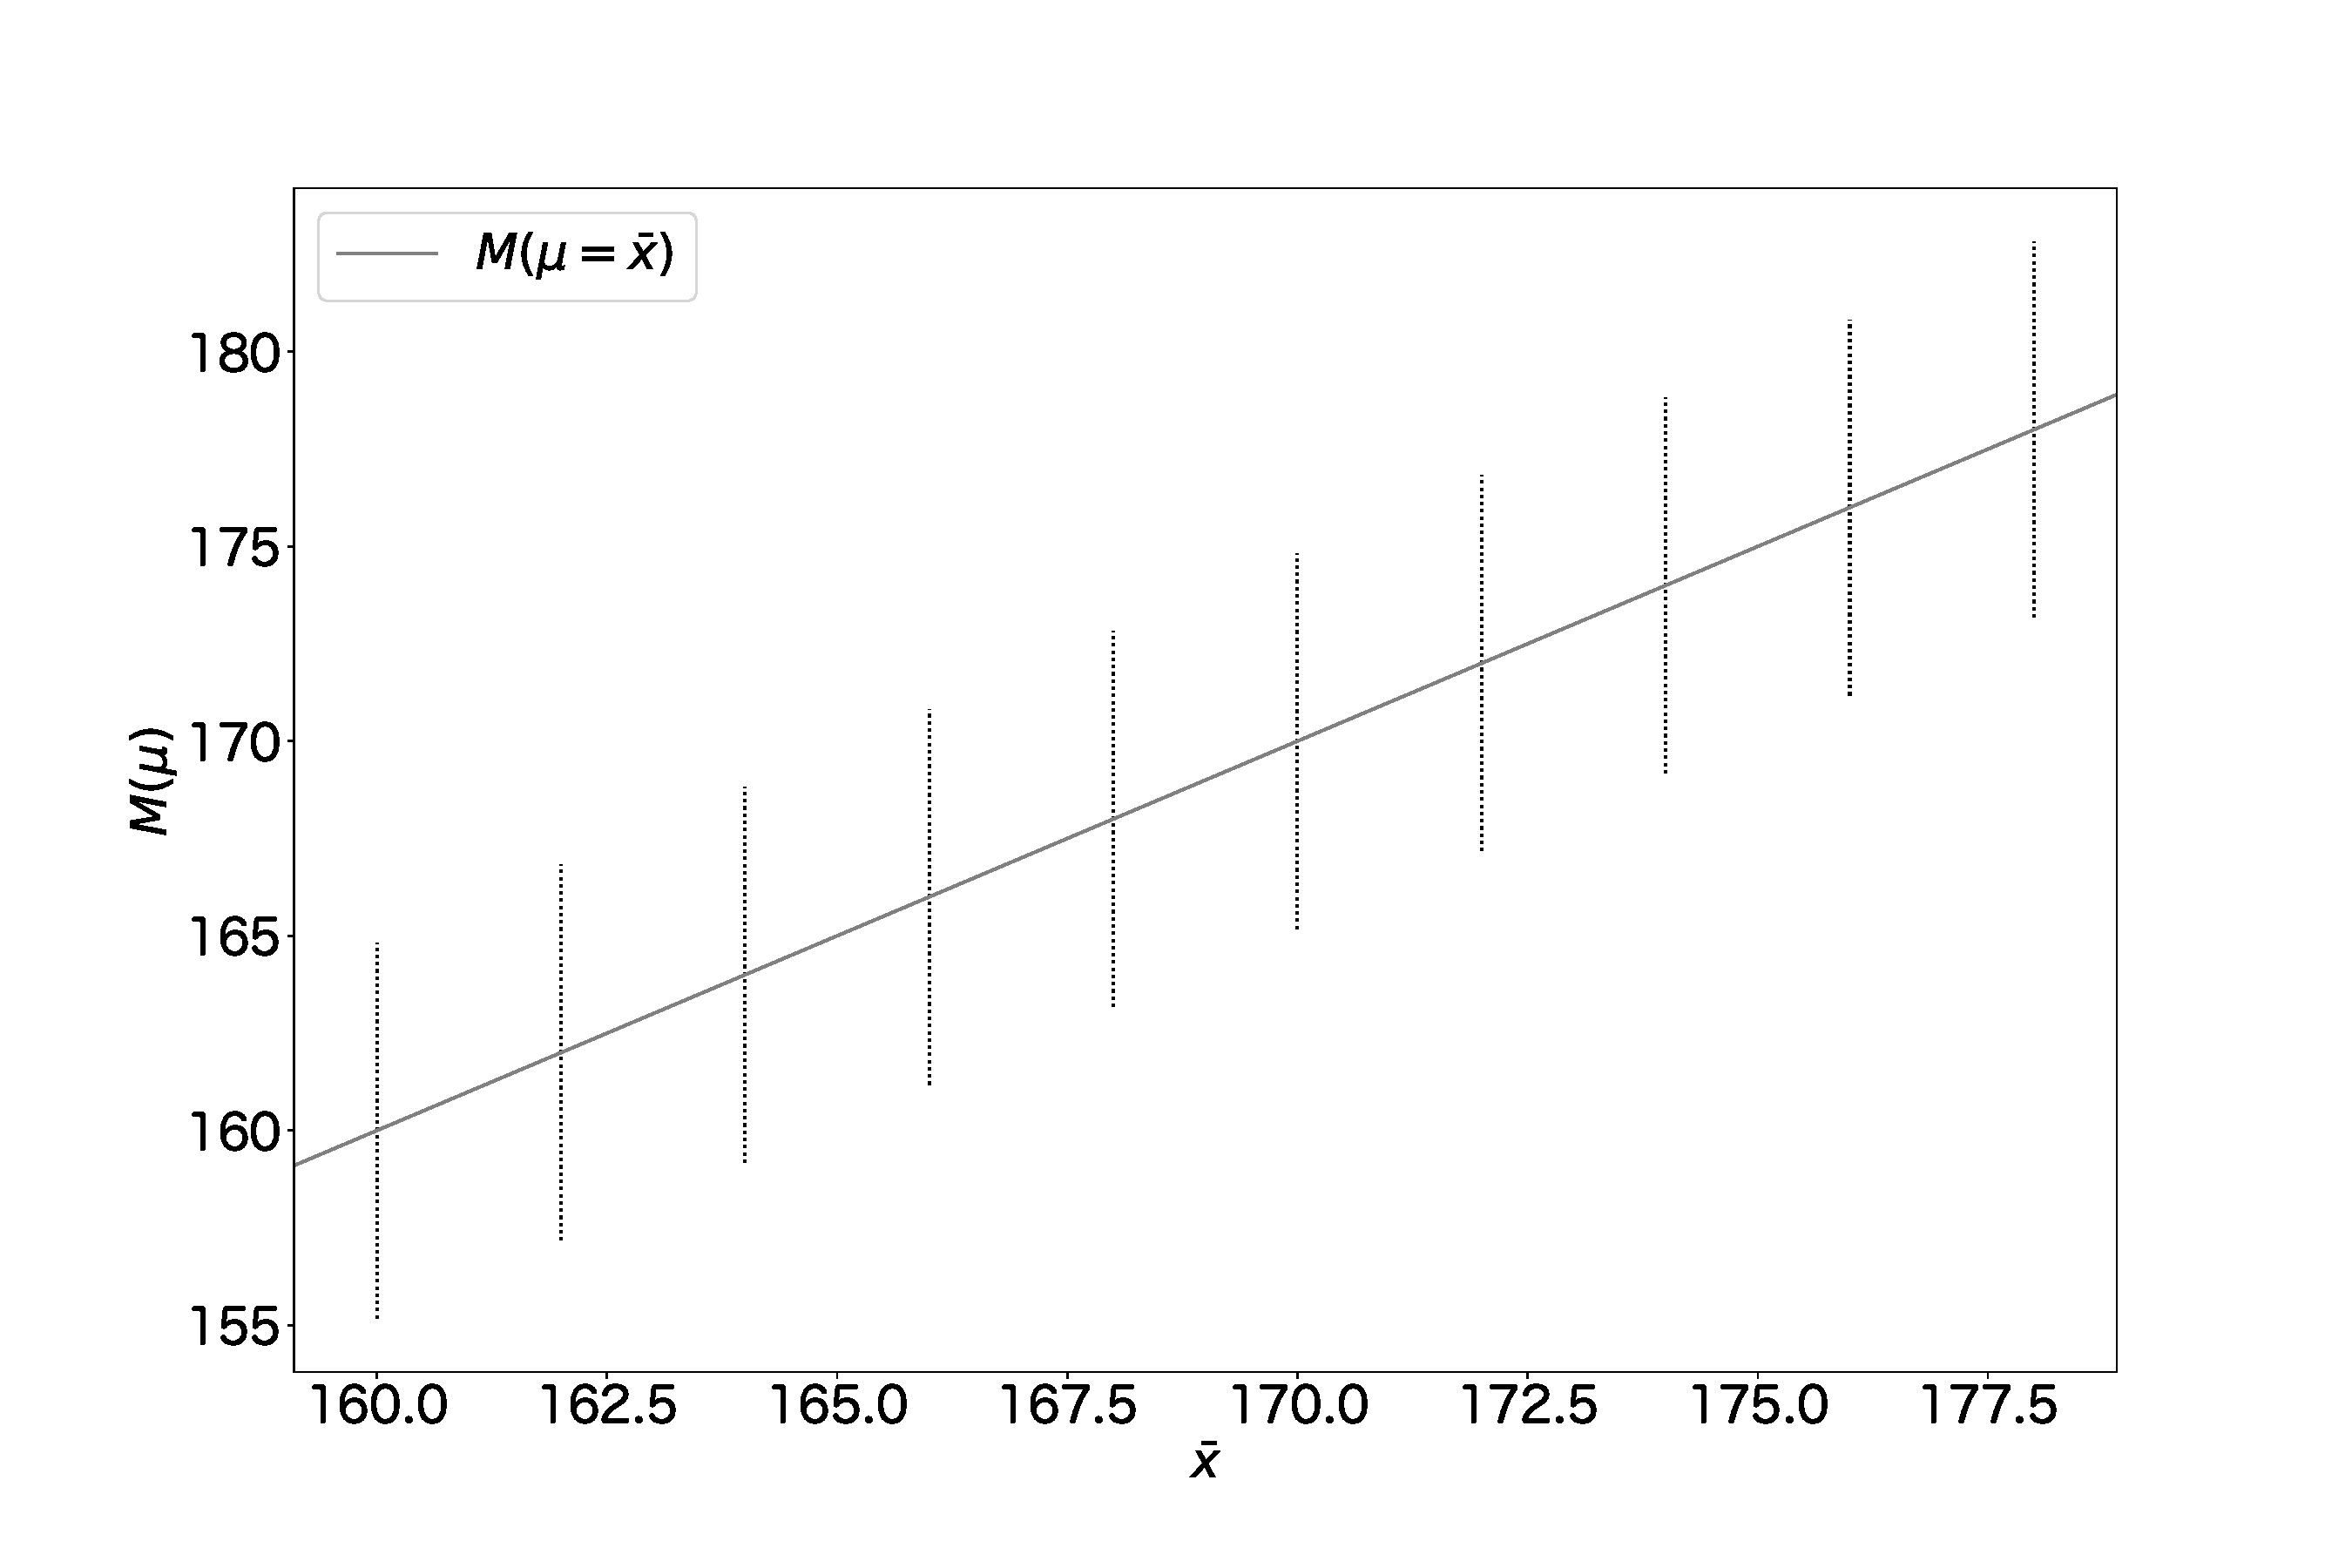
\includegraphics[width=10cm]{./image/04_/confidence_interval_model.pdf}
        \caption{横軸にモデルの母数$\mu$、縦軸に、モデルが予測する平均値$\bar{x}$、エラーバーに$95\%$信頼区間を描いた。$N=10,\sigma^2=6.8^2$}
        \label{fig:confidence_interval_model}

    \end{center}
\end{figure}



\section{統計量をもとにしたモデル間類似度(検出力)}
母数の異なる二つの統計モデル$M_a,M_b$について考察する。
$M_a$の信頼区間内の統計量が$M_b$において出現する確率を検出力という。
言い換えれば一方で出現する統計量が他方のモデルにおいて出現する確率である。
これは、$M_a$から$M_b$へのモデル間の統計量を元にした類似度と言える。

\subsection{検出力の定義}
$M_a$の棄却できない統計量の範囲(信頼区間$A$)に$M_b$の統計量が出現する確率を$\beta$とする。$\beta$を検出力という\footnote{検出力を検定力または統計力と呼ぶこともある。\\ \url{https://id.fnshr.info/2014/12/17/stats-done-wrong-03/}}。
%$\alpha$は統計モデルとデータを比較したとき、そのモデルを棄却する指標である。
$\beta$は、二つの異なるモデルを比較するための指標で、一方のモデルで棄却できない母数がもう一方のモデルで出現する確率である。
$M_a$に対する$M_a$の検出力$\beta$は、$1-\alpha$であり、$M_a$を棄却する閾値を低く設定すると、$\beta$は大きな値になる。
二つの統計モデルの母数がよく一致するならば、$\beta$は$1-\alpha$に近い値を取り、一致していないならば、$\beta$は0に近い値を取る。
具体的に、$\alpha,\beta$を式で書くと、
\begin{eqnarray*}
    & &P_a(x \in R_a) = \alpha\\
    & & P_b(x \in A_a) = P_b(x\notin R_a )=\beta
\end{eqnarray*}
ここで、$R_a,A_a$はそれぞれ統計モデル$M_a$の棄却域、信頼区間、$P_a,P_b$は、それぞれ統計モデル$M_a,M_b$における統計量に関する確率密度関数。

\subsection{正規分布モデルの検出力}
具体的に、$P_a(x \in R_a),P_b(x \in A_a)$を計算してみる。
\if 0
正規モデルを構築する
\begin{quote}
    \begin{enumerate}[(1)]
\item i.i.d
\item $N(\mu,\sigma^2)$
\item 母数$\mu$。$\sigma$は既知とする(一般性を持たせるために、具体的な値は書かない。$\sigma=1$と読み替えて進めても良い)
\end{enumerate}
\end{quote}
\fi
$\sigma^2$がすでに与えられた正規モデルを$M(\mu)$とし、$M_a=M(\mu_a),M_b=M(\mu_b)$とする。
$M_a$または、$M_b$からサンプリングされた確率変数$x_1,x_2,\cdots,x_n$の平均値は、それぞれ$\bar{x}_a\sim N(\mu_a,\sigma/n)$または$\bar{x}_b\sim N(\mu_b,\sigma/n)$である。
$M_a$の信頼区間$A_a$は、$|\bar{x}_a|<\mu_a+\sigma / \sqrt{n}z_{2.5\%}$である。
このとき、$P_a$を$N(\mu_a,\sigma)$の確率密度関数とすると、
\begin{equation*}
    P_a(x \in A_a) = \alpha
\end{equation*}
であるのは定義から明らか。
また、$P_b$を$N(\mu_b,\sigma)$の確率密度関数とすると、
\begin{equation*}
    P_b(x \in A_a ) = \beta
\end{equation*}
である。
$\mu_a$と、$\mu_b$が一致していれば、$P_b(x \in A_a ) = 1-\alpha$である。
$\mu_b$が$\mu_a$から離れていくと、$P_b(x \in A_a)=0$に近づいていく。


\begin{figure}
\begin{center}
    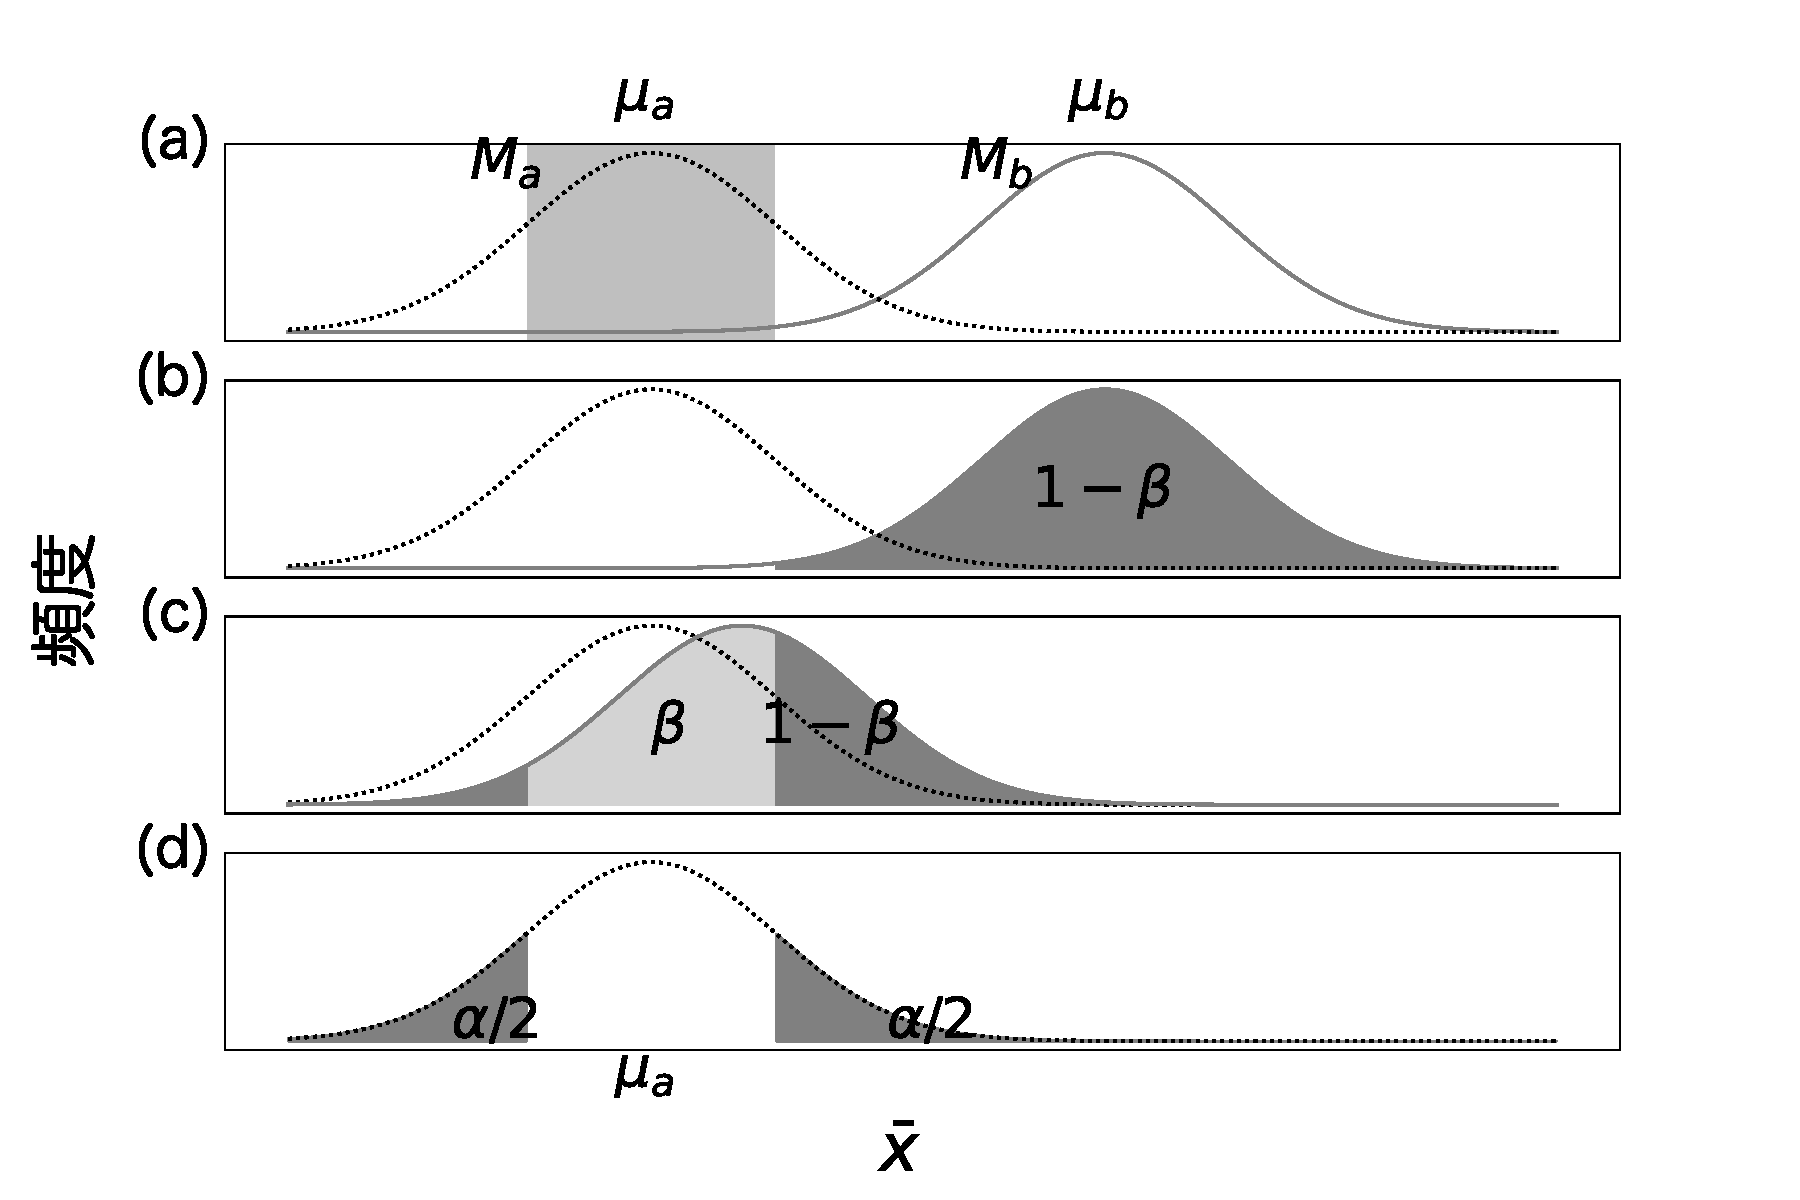
\includegraphics[width=15cm]{./image/04_/power_of_a_test_2.pdf}
    \caption{統計モデル$M_a,M_b$から計算された統計量$\bar{x}$の確率分布$P_a,P_b$。(a)灰色の範囲は$M_a$の信頼区間。(b)灰色の領域は、$1-\beta$の領域を示している。$\beta$の領域が小さいので、描画できなかった (c)$\mu_b$が$\mu_a$に近いときの$\beta$と$1-\beta$の領域。(d)灰色の範囲の面積が$\alpha$を示している。}
    \label{fig:power_of_test_alpha_beta}
\end{center}
\end{figure}


検出力と$\alpha$の領域を図示した(図\ref{fig:power_of_test_alpha_beta})。$M_a$の$95\%$信頼区間は、$|\mu|<\mu_a+z_{0.025}\frac{\sigma}{\sqrt{N}}$である。信頼区間は、図\ref{fig:power_of_test_alpha_beta}(a)において灰色で塗った$x$軸の範囲である。$\alpha$は図\ref{fig:power_of_test_alpha_beta}(c)の灰色で塗りつぶした領域の面積である。
検出力$1-\beta$は、$M_b$における$M_a$の信頼区間の外側の領域の面積なので、図\ref{fig:power_of_test_alpha_beta}(b)の濃い灰色の範囲である。

$\alpha$を0に近づけていくと、信頼区間は徐々に大きくなり、$\beta$は大きくなる。
$\alpha$を1に近づけていくと、信頼区間は徐々に狭くなり、$\beta$は小さくなる。



\begin{figure}
    \begin{center}
        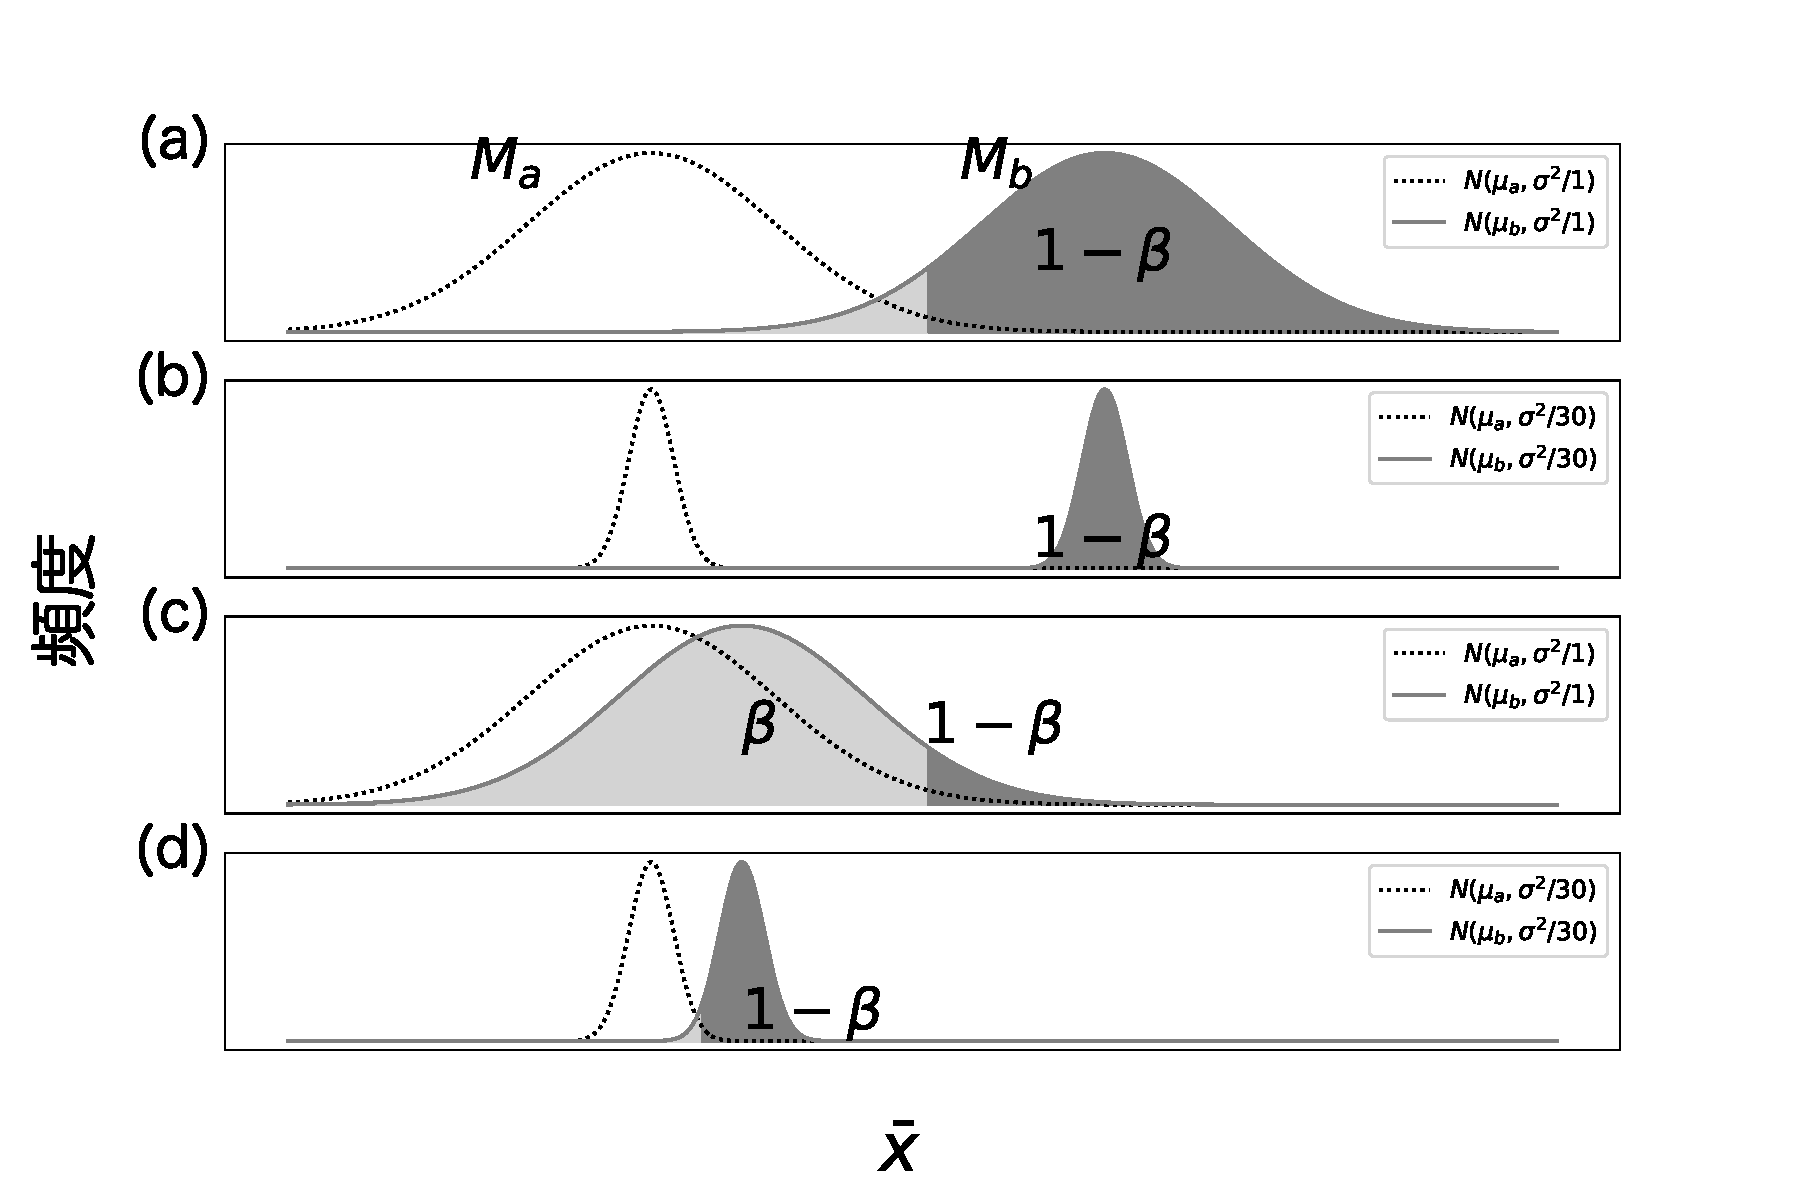
\includegraphics[width=15cm]{./image/04_/power_of_a_test_3.pdf}
        \caption{統計モデル$M_a,M_b$から計算された統計量$\bar{x}$の確率分布$P_a,P_b$。(a)$\mu_a,\mu_b$のサンプルサイズ$1$の平均値がしたがう確率密度関数$N(\mu_a,\sigma^2/1),N(\mu_a,\sigma^2/1)$。(b)(a)と同じ$\mu_a,\mu_b$に対して、サンプルサイズを$30$にした場合の確率密度関数。(c)$\mu_a,\mu_b$が(a)よりも近いときの$\bar{x}$の確率密度関数。(d)(c)と同じ$\mu_a,\mu_b$に対してサンプルサイズを$30$にした場合の$\bar{x}$の確率密度関数。}
        \label{fig:power_of_test_alpha_beta_sample_size}
    \end{center}
    \end{figure}

    

$\alpha$、$M_a$の母数$\mu_a$、$M_b$の母数$\mu_b$を固定したまま、サンプルサイズを変化させ,
$\beta$の変化を表す(図\ref{fig:power_of_test_alpha_beta_sample_size})。$\bar{x}$の確率密度関数($N(\mu,\sigma^2/n)$)の分散がサンプルサイズによって変化することは明らかである。このことから、サンプルサイズが大きくなると、信頼区間は徐々に狭くなり、$1-\beta$は大きくなる。サンプルサイズが小さいときは、$1-\beta$も小さくなる。

$\mu_a$を固定し、$\mu_b$を変化させたときの検出力$1-\beta$を図\ref{fig:power_of_test_N_mu0_variable}に示した。
サンプルサイズが大きければ、$1-\beta$も大きくなることがわかる。

\begin{figure}
    \begin{center}
        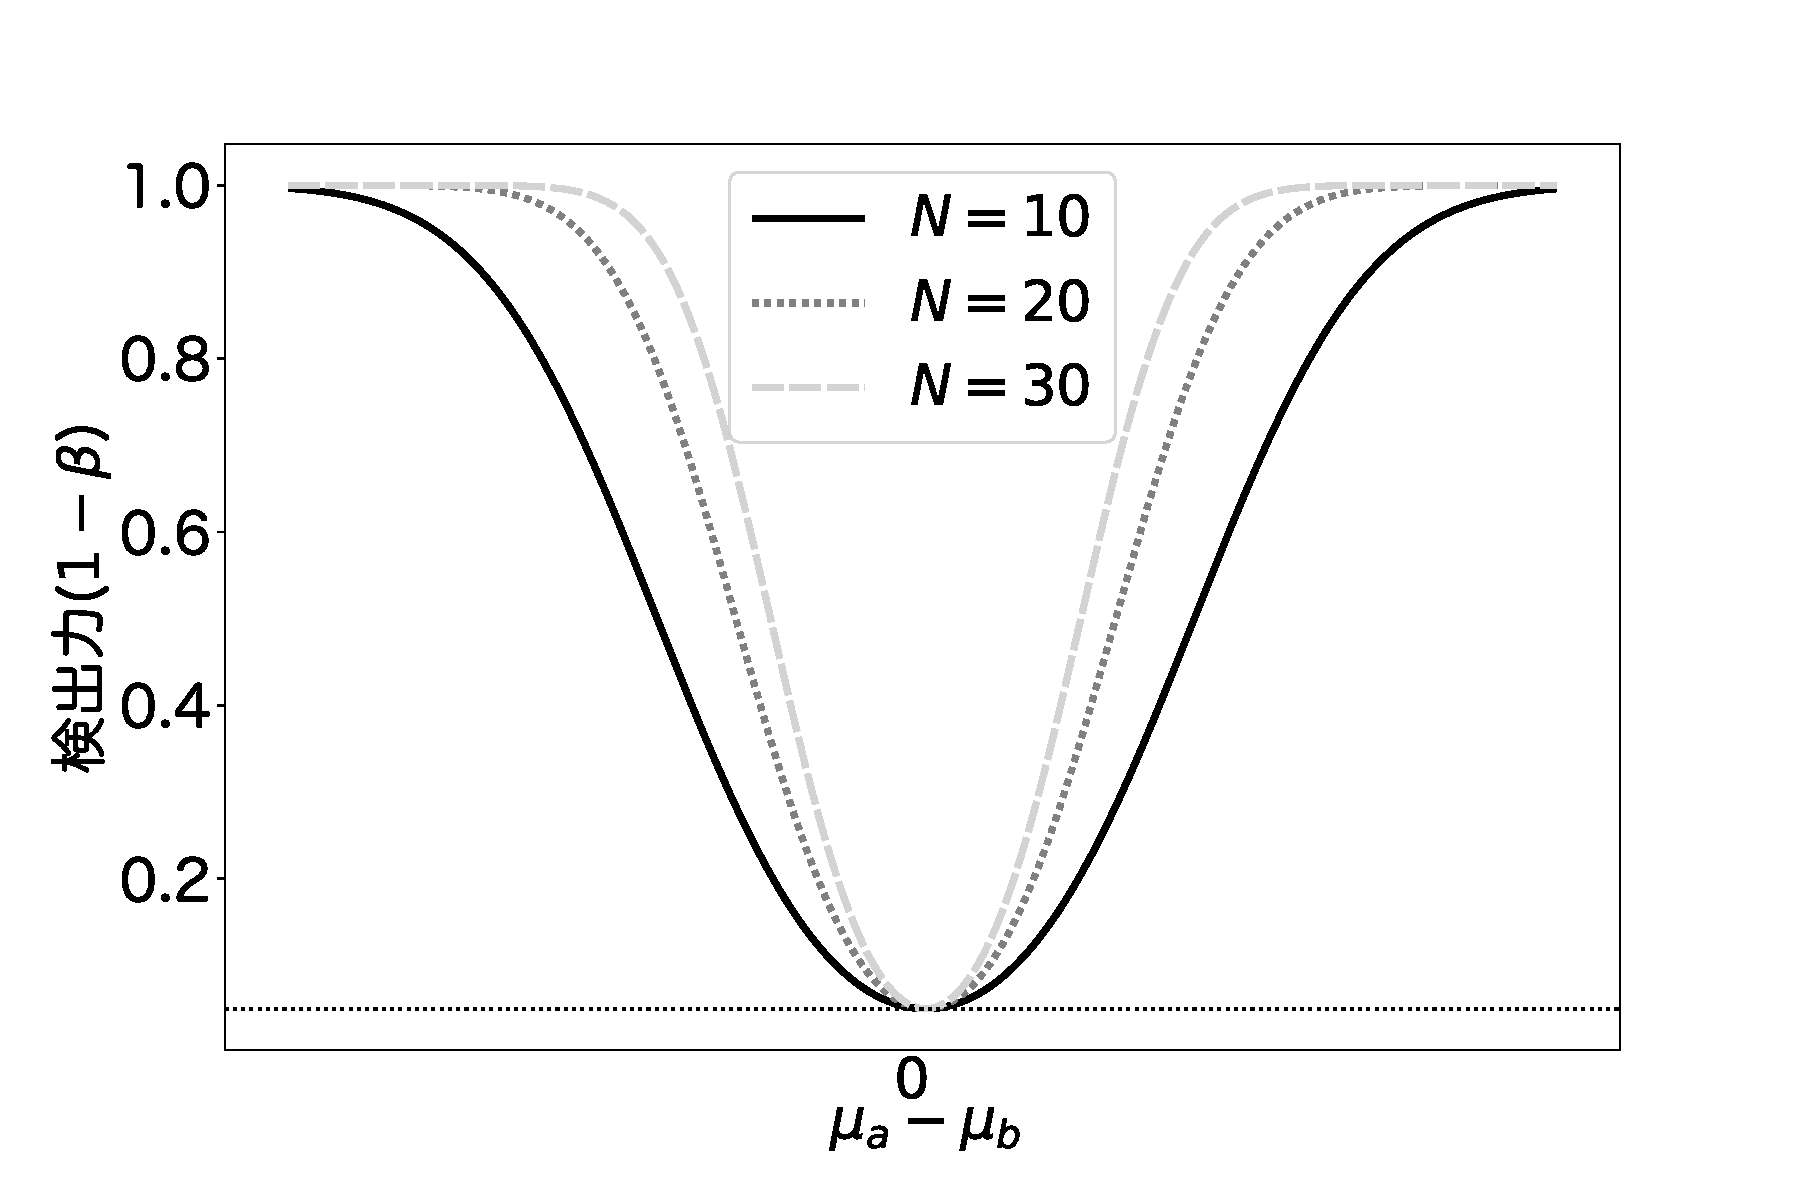
\includegraphics[width=15cm]{./image/04_/power_of_test.pdf}
        \label{fig:power_of_test_N_mu0_variable}
        \caption{$\mu_a$を変数にしたときの検出力(検出力関数)。}
    \end{center}
\end{figure}

$\beta$を定義したことにより、$\beta$の数値を決定し、$M_a,M_b$の違いが$\beta$になるために必要なサンプルのサイズが推測できる。ここでは、$\mu_a,\mu_b$が固定されている状況を考える。
検出力$1-\beta$は$1$に近いほど、$M_a,M_b$が違うと主張できる。
あらかじめ決めたおいた基準の$1-\beta$を閾値を設定し、それ以上の$1-\beta$となるサンプルサイズを推測する。
サンプルサイズが小さければ、$M_a$と$M_b$の違いは曖昧であり、サンプルサイズが大きくなると、はっきりとモデルの違いがわかる。




\subsection{$\beta$の計算}
正規モデル$M_a,M_b$を使って、$\beta$を計算してみる。
$M_a$の信頼区間は、
\begin{equation*}
    -z_{0.025}\leq \frac{\sqrt{n}(\bar{x}-\mu_a)}{\sigma}\leq z_{0.025}
\end{equation*}
より、
\begin{equation*}
    A_a = \{ x ; \mu_a -\frac{\sigma}{\sqrt{n}}z_{0.025} \leq x \leq \mu_a +\frac{\sigma}{\sqrt{n}}z_{0.025} \}
\end{equation*}
である。ここで、$a=\mu_a -\frac{\sigma}{\sqrt{n}}z_{0.025},b = \mu_a +\frac{\sigma}{\sqrt{n}}z_{0.025} $とおく。棄却域は$A_a$以外の$\mu$である。$M_b$の標本平均$\bar{x}_b$は、$N(\mu,\frac{\sigma^2}{n})$に従うので、$A_a$の区間で、$N(\mu_b,\frac{\sigma^2}{n})$の面積を計算すれば良い。
ここで、$\frac{\sqrt{n}(\bar{x}_b-\mu_b)}{\sigma}\sim N(0,1)$である。
このことを利用すると、
$a,b$は、$N(\mu_b,\frac{\sigma^2}{n})$の確率変数だとすると、
\begin{eqnarray*}
    A &=& \frac{\sqrt{n}(a-\mu_b)}{\sigma} \\
    %&=& \frac{\sqrt{n}(\mu_a-\frac{\sigma}{\sqrt{n} z_{\alpha/2}})}{\sigma}\\
    &=& -z_{\alpha/2}+\frac{\sqrt{n}}{\sigma}(\mu_a-\mu_b)
\end{eqnarray*}
同様に、
\begin{eqnarray*}
    B &=& \frac{\sqrt{n}(b-\mu_b)}{\sigma} \\
    %&=& \frac{\sqrt{n}(\mu_a-\frac{\sigma}{\sqrt{n} z_{\alpha/2}})}{\sigma}\\
    &=& z_{\alpha/2}+\frac{\sqrt{n}}{\sigma}(\mu_a-\mu_b)
\end{eqnarray*}
である。以上より、確率密度関数$N(0,1)$において、$-z_{\alpha/2}+\frac{\sqrt{n}}{\sigma}(\mu_a-\mu_b) \leq x\leq  z_{\alpha/2}+\frac{\sqrt{n}}{\sigma}(\mu_a-\mu_b)$の間で積分すれば良い。

$d=\frac{\mu_a-\mu_b}{\sigma}$とおく。$d=0.6,n=9$とする。このときの$\beta$を計算してみる。$N(0,1)$において、$-z_{\alpha/2} -0.6\sqrt{n} \leq x \leq z_{\alpha/2} +0.6\sqrt{n}$の区間で積分する。

\begin{lstlisting}
A,B = norm.interval(0.95,0.,1)
N = 9
d = 0.6
a,b = A+d*np.sqrt(N),B+d*np.sqrt(N)
print(a,b)
norm.cdf(b,0,1)-norm.cdf(a,0,1)
\end{lstlisting}

答えは、$0.564$


\subsubsection{サンプルサイズ}
$d$と検出力を指定したときに、$M_a,M_b$の類似度を検出力以上にするためのサンプルサイズが計算できる。
$\beta=0.1,\d=0.8$とし、この$\beta$を満たすように$N$を計算した。

\begin{lstlisting}
A,B = norm.interval(0.95,0.,1)
beta = 0.1
d = 0.8
for N in range(10,200,2):
    a,b = A+d*np.sqrt(N),B+d*np.sqrt(N)
    beta_ = norm.cdf(b,0,1)-norm.cdf(a,0,1)
    if beta_ < beta:
        break
print(N)
\end{lstlisting}
計算を実行すると、$18$であることがわかる。



\subsection{最尤モデルでの$\beta$の計算}
\subsubsection{データを元にしたモデルとモデルの類似度}
統計モデルAを$M(\mu=170)$とし、統計モデルBを$M(\bar{X})$とする。ここで、$\bar{X}$は、無作為抽出によって得られた標本の平均であり、標本の大きさを$100$とする。
モデルA,Bの間の検出力が計算可能である。
$d=\frac{170-\bar{X}}{6.8}$、$n=100$であるので、$\bar{X}=168$を得たとすると、
\begin{lstlisting}
A,B = norm.interval(0.95,0,1)
N = 100
d = (170-168)/(6.8)
a,b = A+d*np.sqrt(N),B+d*np.sqrt(N)
print(a,b)
norm.cdf(b,0,1)-norm.cdf(a,0,1)
\end{lstlisting}
その検出力は、$0.163$


\section{過誤}
これまでの議論をまとめる。モデル$M_a$からサンプリングを行った標本について、モデル$M_a$に関する標本であるかを判定する。モデルから生成された標本であるが、偏った統計量出会った場合は、モデルから生成されていないと判断する。この頻度を$\alpha$とした。このように、モデル$M_a$から生成されたのに、統計量の出現頻度から、このモデルから生成したものではないと言う誤った判断を行う事になる。このことを判断の間違いであると言うことから第1'の過誤と呼ぶ\footnote{Neyman-Pearsonとは異なる過誤を定義したので、1'および2'とした。仮説検定において、Neyman-PearsonとFisherを混ぜ合わせて過誤を定義することが現在の主流である。こちらの定義では、さまざまな誤解が生じている\cite{1573106361610039296}}。

今度は、モデル$M_b$からサンプリングを行った標本が、別のモデル$M_a$からサンプリングされたかを判定する。統計量が信頼区間に入っているかどうかを確認し、入っていなければ、モデル$M_a$からサンプリングされていないと判定できる。問題が生じるのは、統計量が信頼区間に入っている場合である。これは、実際には、$M_a$からサンプリングされていないのにもかかわらず間違って、サンプリングされたと判断する事になる。この判断の間違いを第2'の過誤と呼ぶ。

\begin{table}[hbtp]
    \caption{モデル$M_a$による自己標本批判}
    \label{table:type_error}
    \centering
    \begin{tabular}{ccc}
      \hline
        &  $M_a$の信頼区間に &  $M_a$の信頼区間に \\
        & 標本の統計量が入っていない & 標本の統計量が入っている \\
      \hline \hline
      モデル$M_a$の標本  & モデル$M_a$の標本ではないと判定  & モデル$M_a$の標本と判定 \\
      & (第1'の過誤) & \\
      モデル$M_b$の標本  & モデル$M_a$の標本ではないと判定   & モデル$M_a$の標本であると判断 \\
      & & (第2'の過誤) \\
      \hline
    \end{tabular}
  \end{table}

  \begin{SMbox}{過誤はデータとモデルを比較したときに生じる判断ミス}
  データとモデルを比べたときに、誤ってモデルが間違いと判定することを第一の過誤と教科書において紹介していることがある。誤ってモデルが間違いと判断するとはどのようなことなのかの定義がないので、この定義の意図がわからない。

  本書では、モデルからサンプリングした標本とモデルを比較したときに生じる間違いとして過誤を定義した。標本は無作為抽出によって得られたものではない。
  \end{SMbox}


\begin{SMbox}{正解と回答の違い}
    あるデータ群に対してそのデータの特徴を元に、YesまたはNoとアノテーションをつける。
    データからそのYesまたはNoを予測する手順を開発する。
    その手順によって得た回答と、正解(真の値)の一致と不一致は以下の通りになる(表\ref{table:Yes_no_answer})。
    回答と一致したら、True、一致しないならFalse。
    Yesと予測したらPositive、Noと予測したらNegativeとする。
    回答がYesな問題に、Yesと答えることは(手順が正しい予測を行なった)、True Positiveといい、Noと答える(手順が間違えた予測を行なった)ことはFalse Negativeという。回答がNoな問題に、Yesと答えることを、False Positive、また、Noと答えることをTrue negativeという。

    モデル$M_a$の標本にYesを対応ずけ、モデル$M_b$の標本にNoを対応付ける。標本を元に、YesまたはNoを判定する手順をモデル$M_a$を元にした統計検定を利用する。この問題において回答がFPとなったものを第1'の過誤であり、FNとなったものが第2'の過誤である。
    \end{SMbox}
    
    
    \begin{table}[hbtp]
    \caption{正解と回答の違い}
    \label{table:Yes_no_answer}
    \centering
    \begin{tabular}{ccc}
        %\hline
          &  負例(真の値) & 正例(真の値)  \\
        \hline \hline
        正例(予測値) &  偽陽性(FP)  & 真陽性(TP)\\
        &予測が外れた & 予測が当たった\\
        負例(予測値) & 真陰性(TN) & 偽陰性(FN)\\
        & 予測が当たった & 予測が外れた\\
        \hline
    \end{tabular}
    \end{table}

    

\begin{SMbox}{$p<\alpha$なら違うことがわかる}
    %もともと違うことは実験設定から明らかである。
    モデルの上でも、モデル由来の標本であるかどうかはわからない。
\end{SMbox}


\section{自己否定の過推定}
統計モデルの中で、統計モデルを統計量により検査するときに、モデル自身を絶対にダメなモデルと判断しすぎてしまうことを自己否定の過推定と言う。
この過誤は2つの要因に分解でき、\footnote{$\alpha_2$は$\alpha_1$に関係するので実際には、分解できない。気持ちとしては、$\alpha_2$は、$\alpha_1$を変数に持つ関数である$\alpha=\alpha_2(\alpha_1)$。}、不適切な統計量を使用することで、棄却域と統計量の違いにより生じる$\alpha_1$、そして、検定を繰り返して生じる$\alpha_2$である($0<\alpha_2 \leq 1$)。
$\alpha_2=\alpha$となっていれば、有意水準$\alpha$の検定ができる。
$\alpha_1$は、統計モデルと、その統計量の関数になっており、言い換えれば、統計量が統計モデルの中で設計通りの振る舞いをしているかを測る指標である。
正規モデルを使い、統計量$T$を使った場合、$\alpha_1 \approx	 0 $であるが、指数モデルを使い、統計量$T$を使った場合、$\alpha_1$が指定した$\alpha$よりも多くなる。これを見ていく。
$\alpha_2$は、$\alpha\times 2$以上になる場合、軽視されることはないが、
$\alpha_1$が同程度の隔たりになる場合においては無視され、$\alpha_1$は$\alpha_2$よりも軽視されがちであることも説明する。
%統計モデルに対して不適切な統計量を使ってモデルの検証を試みると、第一の過誤が変化することがわかっている。




\subsection{どんな統計モデルでも$T$統計量で調べよう($\alpha_1$)}
統計モデルの分布の仮定が正規分布以外の場合においても、$T$統計量を使ってモデル自身を検証できるのかを調べる。次の統計モデル$M_E(\lambda)$を構築する。
\begin{enumerate}
    \item $X_1,X_2,\cdots,X_n $はi.i.d
    \item 指数分布
    \item $\lambda$
\end{enumerate}
母数$\lambda=1$とした統計モデルを$M_E(1)$とする。
$M(1)$からランダムサンプリングした確率変数$x_1,x_2,\cdots,x_n$から次の統計量を計算する。
\begin{equation*}
    T = \frac{\bar{X}-1}{\sqrt{\frac{\sigma^2}{n}}}
\end{equation*}
ここで、$T \sim t(n-1)$とする。
$T$値が$t(n-1)$の棄却域に入っている頻度を数値計算により計算する。
具体的に、平均$1$の指数分布または、平均$1$、標準偏差$1$の正規分布からサンプルを得て標本を作る。その標本を$100000$回取得する。
このとき、$T$値を計算し、$T$値いじょの値が得られる確率$p$を計算する。その$p$が$p<0.05$となる割合を計算する。以上をサンプルサイズを変化させてシミュレーションを行なった。
平均$1$、標準偏差$1$の正規分布の場合、$T$値は$t(n)$分布に従ので、$p<0.05$となる頻度も、$5\%$程度になることが期待される。
一方で、平均$1$の指数分布の場合、$T$は$t(n-1)$分布に従うとはいえない。このことから、$p<0.05$となる頻度は計算してみなければわからない。


\begin{figure}
    \begin{center}
        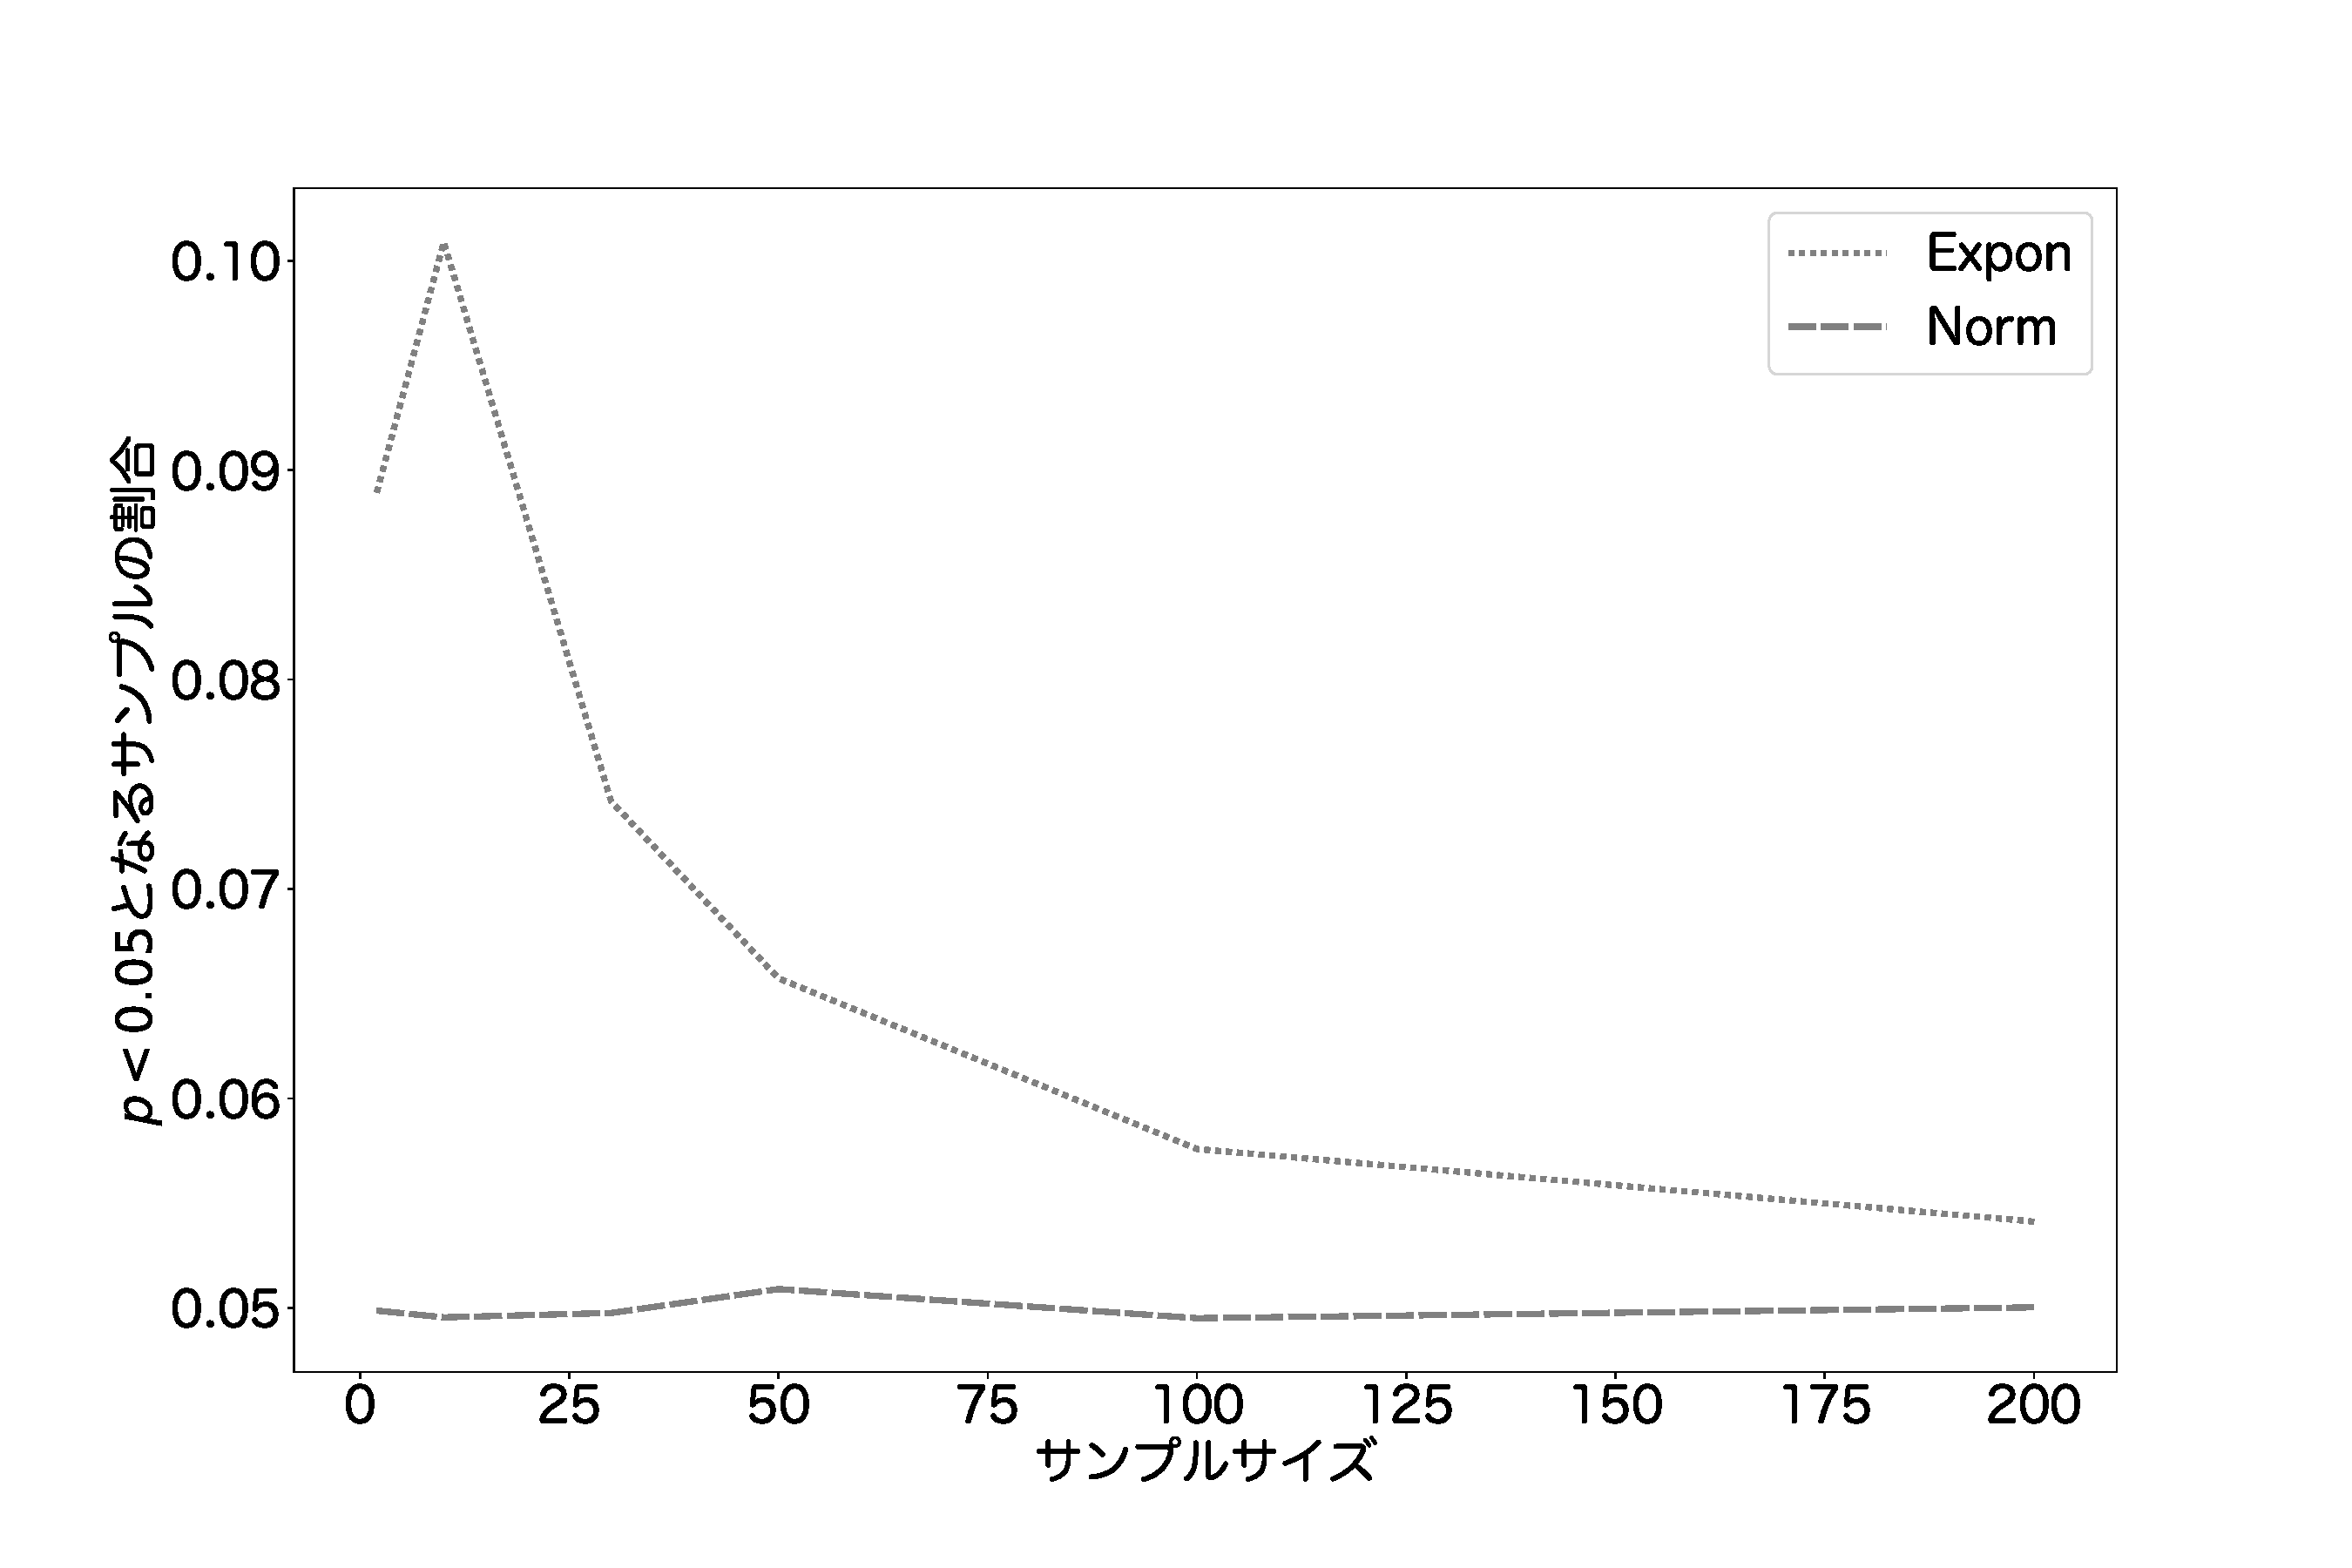
\includegraphics[width=15cm]{./image/04_/t_test_expon_norm.pdf}
        \caption{正規分布または指数ぶんぷから得た標本の$T$値から計算した$p$値で、$p<0.05$以下になる割合}
    \end{center}
\end{figure}

シミュレーションの結果、正規分布から標本を得た場合、$p<0.05$になる割合は、サンプルサイズに依存せず、$5\%$程度であり、期待通りである。
一方で、指数分布から標本を得た場合、$p<0.05$になる割合はサンプルサイズに応じて変化しており、また、どのサンプルサイズでも$p<0.05$となる割合は$5\%$より多い。

このことから、指数モデルの$\alpha_1$は、$\alpha_1>0.05$であることがわかり、統計量を正しく選ばなかったことで、自己否定の過誤が期待した$0.05$よりも大きくなっていることがわかる。


\begin{SMbox}{サンプルサイズがxx以上あるから$t$検定}
        サンプルサイズがある値以上あるので、中心極限定理により、$t$検定が利用できるというものもある\footnote{http://id.ndl.go.jp/bib/024660739}。このロジックが読み込めなかったので、その謎を明らかにすべく我々はアマゾンの奥地へ向かった。

        %サンプルサイズが1以上であれば、$t$検定を行うことは原理的には可能である。
        データが指数分布的であるときに、$t$検定を使うときに生じる問題は上でみた通りであり、$p<0.05$となる標本の割合が多くなっているので、間違った推測をする可能性が高くなる。
        他の分布関数でもおそらく同じような現象が現れる。
        このことから、我々は「$t$検定が利用可能である」は正確ではなく、「$t$検定を使うことができるが、間違った推測である確率が高くなる」ということだと推察した。

        %サンプルサイズが大きくなれば、$\alpha_1$は小さくなる。
        業界によっては、サンプルサイズが$xx$以上であれば、過誤を無視して良いというふうに言われることもある。実際には、設計したモデルと
\end{SMbox}

\section{検定を繰り返し使おう($\alpha_2$)}
ここまでは、一つの標本に対して、統計モデル$M(\mu)$により推測できるかを考えていた。
ここでは、$\sigma^2=10^2$とした正規モデル$M(\mu)$によって複数の標本について推測できるかを仮説検定を指標にし考える。
%ここでは、複数の標本について、$M(\mu)$により推測できるかを
標本が$3$個あるとする。このとき、それぞれの標本の統計量$T$が信頼区間に入っている確率は、$(1-\alpha)$である。全ての標本の統計量$T$が信頼区間に入っている確率は、その積$(1-\alpha)\times(1-\alpha)\times(1-\alpha)=(1-\alpha)^3$であり、この確率で統計モデルは棄却されない。
一方で、棄却される確率は、$1-(1-\alpha)^3$である。
\begin{table}[hbtp]
    \caption{標本数に応じた$\alpha_2$}
    \label{table:multiple_test_reject_prob}
    \centering
    \begin{tabular}{lcr}
      \hline
      標本数  & $\alpha=0.05$  &  $\alpha=0.01$ \\
      \hline \hline
       1 & $0.05$  & $0.01$ \\
       2 & $0.0975$ & $0.0199$\\
       3 & $0.142$ & $0.0297$\\
       4 & $0.185$ & $0.0394$\\
    \end{tabular}
  \end{table}
表\ref{table:multiple_test_reject_prob}は、標本数に応じた$\alpha_2$である。標本数が大きくなるについれて、$\alpha_2$が大きくなることがわかる。

$\alpha_1$がレベル$\alpha$の検定になっていない場合、$\alpha_2$はさらに有意水準$\alpha$から隔たりの多い数値になる。




\section{類似度の過誤}
統計モデルの間の類似度を検出力といった。
統計モデルに対して、不適切な統計量を与えたとき、検出力を歪める。
これを類似度の過誤といい、その確率を$\beta'$で表す。
直接またはシミュレーションを行い$\beta$を計算することがおそらくできそうだが、面倒なので行わない。



\section{データとモデルの比較}
ここで、いくつかのことを定義しておく。
\begin{defi}
    統計モデルと標本を比較して、モデルが母集団のことを予測できないとさまざまな指標をもとに判断するとき、統計モデルを却下すると宣言する。
    %ある標本から求められた統計量以上に大きな値が得られる確率を$p$値と呼ぶ。
    %絶対にダメと判断されないときは、統計モデルを採択(棄却の対義語)すると宣言しない。
    %統計モデルが棄却されるのは、統計モデルの仮定によって変化する。本書の範囲内であれば、統計モデルの母数、分布関数、独立同一の分布関数からサンプリングされたことによる。
    %最尤統計モデルにおいて、棄却されない統計モデルの母数の範囲を信頼区間といい、棄却されるモデルの母数の範囲を棄却域という。
\end{defi}
%ある閾値$\alpha$を決めて、それよりも小さな$p$値をもつ標本について、モデルから得られたものではないと判断する。ここで、$\alpha$を有意水準という。

\begin{SMbox}{検定統計量や$p$を計算するだけで解析完了}
    統計検定量があるモデルに適合的かどうかがわかるだけである。
\end{SMbox}


ここで、母集団から無作為抽出した標本(モデルから生成された標本ではない)を正規モデルにより、予測できるかを考える。
上記の議論と同様に、標本から、統計モデルにあった統計量を計算し、統計量よりも偏った値が出現する確率($p$値)を計算する。
$p$値が小さければ、モデルにより予測できないと考え、値が1に近いほど、もしかしたらモデルで予測できるのかもしれないと考える\footnote{$p$値だけで判断してはいけない}。
標本を元に、モデルにより予測ができないかを考えている。
%このとき、モデルを却下すると宣言する。
%$p$値が$\alpha$よりも小さいとき、流石にこのモデルでは予測できないでしょうと判定する。
%$p$値が$\alpha$よりも大きい場合でも、そのままこのモデルで予測できるとは宣言しない。他の指標やデータとモデルをグラフにより比較し、予測できそうかを考察する必要がある。

%この標本は、モデルからサンプリングしたものではない。
%標本の統計量が、モデルの上で得られやすいものかを調べる。
%$M_a$を棄却する判断をする閾値は、言い換えると、統計モデル$M_a$の棄却される母数(棄却域$R$)の出現確率を$\alpha$とした。


以上のことは、托卵行動に例えることができる。
モズは、カッコウに対して卵を託す托卵を行い、カッコウは、モズの卵とは気が付かず、そのまま育てる。
ここで言い換えたいのは、カッコウは統計モデルであり、卵は標本そして、モズは科学者である。
統計モデルは、モデルからのサンプリングされた標本を巣穴に置いている。
卵の情報を要約した統計量が、モデル由来であることをモデルはその統計量の出現頻度を推測できる。
出現頻度が$p$値である。
モデルの巣に自然から無作為抽出した標本を科学者が置く。
その標本の統計量の出現頻度をモデルは推測できる。
得られた推測から、標本がモデルの卵であることを判定するのは科学者である。
この手順だけでは科学者はモデル鳥と標本卵を比較しているだけであり、標本卵を構成しているデータそのものとモデル鳥を比較していないということに注意しなければならない。


\begin{figure}
    \begin{center}
        
\includegraphics[width=15cm]{./image/01_/conceptual_diagram/conceptual_diagram.003.png}
        \caption{統計量を使ったモデルとデータの比較に関する概念図}
        \label{fig:conceptual_diagram_test}
    \end{center}
\end{figure}
    


\begin{SMbox}{偶然の差が生じたかを確かめたい}
    「偶然の差が生じたかを確かめたい」や「こんなことが起こる確率は$5\%$くらい」という言葉を統計学の教科書で見たことがある。これらは、本書での説明とは異なる前提をもとに議論を進めており、本書と解釈の互換性はない。
    %「統計モデルの上で統計量が現れる確率が十分小さいことを確かめたい」や「統計モデル上でそのような統計量が得られる確率が$5\%$」を省略して書いたものです。
    
    科学では、実験で得られたデータは、同様の実験を行った場合、同様のものが得られるということが前提になっている。このことを現象に再現性があると言う。
    再現性のないデータを現状の統計学で扱うことや、現実の現象が得られる確率を議論することは困難である。

    本書の前提を元にすれば、「こんなこと(これ以上に偏った統計量値)が(モデル内で)起こる確率は$5\%$くらい」ということを省略して「こんなことが起こる確率は$5\%$くらい」と言うことはできる。また、現実において起こりやすいのかどうかについては議論できない。
\end{SMbox}


\subsection{$p$値を使った判断に関する注意}
$p$値を元に統計モデルとデータの不一致を考えるとき、$p$値はモデルとデータの乖離を示す指標の一つであると言うことを意識しなければならない。このことを忘れてしまい、次の間違った判断を行うことがある。
\begin{enumerate}
    \item $p$値が0に近いならば、統計モデルによりデータを予測できないと判断する
    \item $p$値が1に近いならば、統計モデルによりデータを予測できると判断する
\end{enumerate}
それぞれのデータがどのようなものなかのかを確認してみる。
\subsubsection{$p$値が0に近い$\rightarrow$統計モデルによりデータを予測できないと判断}

\subsubsection{$p$値が1に近い$\rightarrow$統計モデルによりデータを予測できると判断}




\begin{SMbox}{P値が小さければ、モデルの仮定のうち少なくとも一つが間違い}
    \ 
    \begin{quote}
        P値が小さければ、データと帰無仮説の矛盾している程度が大きいので、P値が小さければ帰無仮説は棄却するんだと統計の教科書には書かれています。実はそうではなくって、今お話ししたように小さいP値が何を意味するかというと、たくさんある統計モデルの仮定のうちどれか一つが間違っているあるいは、複数のものが間違っている。決して帰無仮説だけが間違いの対象ではなくって、先程のように、小さいP値が選択的に報告してあれば、結果としては誤った結果になります。・・・・
        %ランダム化もランダムサンプリングもなされていなければ、そもそも、データに対して確率計算をすることも意味がないことですから、そういうデータでなければ、P値を計算する意味すらなくなってしまう。
        \footnote{京都大学大学院医学研究科 聴講コース 臨床研究者のための生物統計学「仮説検定とP値の誤解」佐藤 俊哉 医学研究科教授 \url{https://www.youtube.com/watch?v=vz9cZnB1d1c} }
    \end{quote}
    P値が小さければ、モデルの仮定のうち少なくとも一つが誤っているというものがある。私はこの意見に賛成できない。

    モデルの中で標本の統計量以上の値の出現確率を計算したものが$P$値である。$P$値によって、仮定の間違いを主張できるような値ではない。ある母数を持つモデルによりデータの平均値を予測できなかったことを示唆すのが$P$値である(パラメトリックモデルの範囲であれば)。
    正規分布や独立同分布ではないことを示唆することはおそらくない。

    ただ、モデルとデータの比較を行なった後、データが目的にあっているのかを調べなければならない。
    %モデルの仮定をデータが満たしていることを$P$値では測れない。モデルの仮定をデータが満たすことはほとんどない。
\end{SMbox}


\begin{SMbox}{モデルの仮定を満たせるのか}
    \ 
    \begin{quote}
    最初の原則。最初に述べられている原則ですが、P値はデータと特定の統計モデルが矛盾する程度を示す指標の一つであるというふうに書かれています。ここでですね、統計モデルは何かって言うと、統計モデルは必ず一連の仮定のもとで構成されています。どんな仮定かと言いますと、統計の教科書をみますと、「データが正規分布している」とか、「平均値が等しい」などが統計モデルに必要な仮定とされているのですが、まず、一番大切なことは、データを撮るときに、先程の試験のように、薬剤のランダム割り当てが行われているとか、対象者を剪定するときにランダムサンプリングがなされているか、こういったことも統計モデルの仮定に含まれています。
    それから当然、研究計画がきちんと守られているかも統計モデルが必要とする前提の一つです。例えば、先程の臨床試験で言えば、
    結果の解釈も変わってきます。最後まで対象者が追跡できているのか。追跡不能とからつだくがあったとすると、統計モデルの後世に影響を与えます。もちろん解析方法も妥当な結果を与える解析方法でなければいけない。
    こういったことを満たしていなければ、統計モデルの仮定を満たしているとは言えない。
    %もちろん、全ての解析結果が報告されている。これは統計モデルに必要な仮定とは言えないですが・・・
    \footnote{京都大学大学院医学研究科 聴講コース 臨床研究者のための生物統計学「仮説検定とP値の誤解」佐藤 俊哉 医学研究科教授 \url{https://www.youtube.com/watch?v=vz9cZnB1d1c} }
    \end{quote}

    この意見は統計モデルに関する仮定と実験計画の二つの要素が混じっている。実験計画を統計モデルの仮定を満たすように設計するという意見だと考えられる。
    この意見に賛成しない。

     まず、統計モデルの仮定が自然において対応するものが、本書においてはない。また、「平均値が等しい」という仮定であるが、ある平均値をもつ統計モデルとデータを比べるさいに、データの平均値が異なる場合においても、統計モデルを使ってそのデータの出現頻度などを推定することが可能である。
     このことは、モデルの仮定をデータが満たさなければならないことを示唆していない。

     次に、実験計画については、科学者がみたい効果を見るために設定しているのもである。ランダムサンプリングしているのは、対象に偏りがないようにし、さまざまな対象である特徴の変化を与え、その集団内での変化を計測するために行う。
     対象の選定に偏りがあった場合、本当に推測したかったことが推測できない。例えば、成人以上を対象にした試験なのに、60歳だけしかからサンプリングできなかったなら、成人に対しての言及はできない。
     また、偏りのあるデータを偏りを前提としていない統計モデルにより解釈するのはこんなんである。
     この困難さを回避するためにも実験デザインを守った無作為抽出であった方が良い。
     
     いずれも本書の方針とは異なる。
     %モデルに対してではなく、科学者がみたいものが見れなくなることを意味する。
     %モデルは偏ったデータが得られたことを考慮して構築していない。
     %モデル自体に偏りを設定すればよいはずであるが、


     %医学における研究が予測精度を高めるということを目的にして統計学を使っていないので、意見が一致しない。
\end{SMbox}
